{Match the following equations to their slope fields.\\
(i) $y'=1-x$\\
(ii) $y'=x-2y$\\
(iii) $y' = x(1-y)$\\
Justify.

\medskip

\begin{tabular}{c}
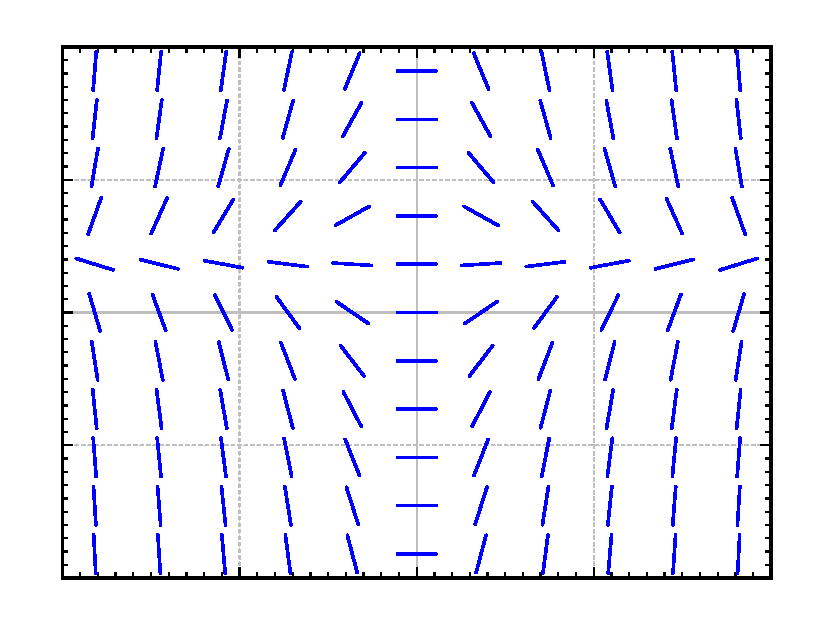
\includegraphics[width=1.5in]{figures/yprimex1minusyslope}\\
(a)
\end{tabular}\\
\begin{tabular}{c}
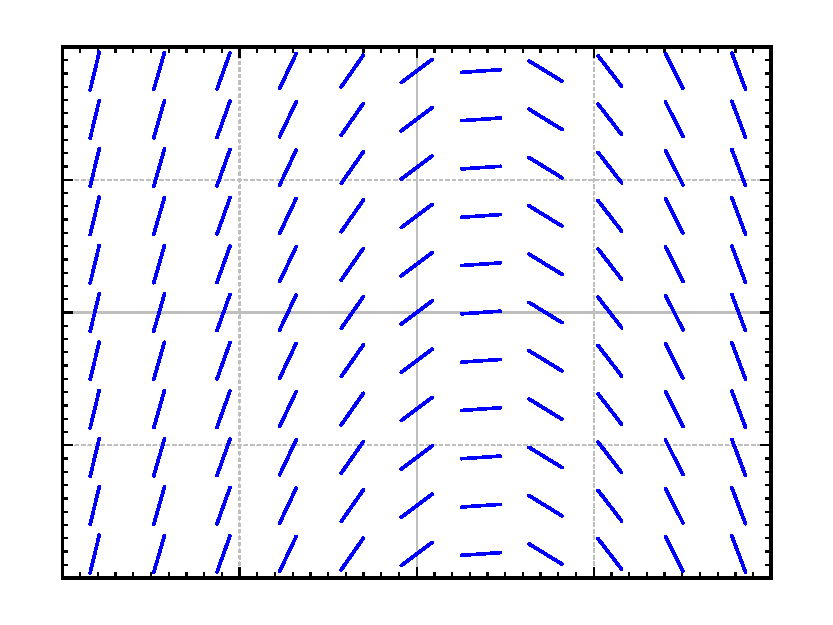
\includegraphics[width=1.5in]{figures/yprime1minusxslope}\\
(b)
\end{tabular}\\
\begin{tabular}{c}
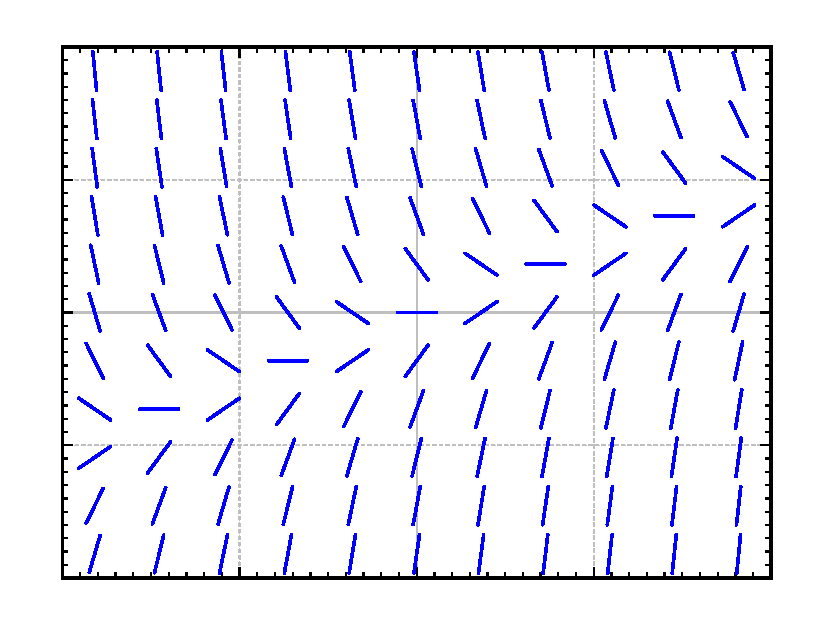
\includegraphics[width=1.5in]{figures/yprimexminus2yslope}\\
(c)
\end{tabular}
}
{Equation (i) corresponds to slope field (b).\\
Equation (ii) corresponds to slope field (c).\\
Equation (iii) corresponds to slope field (a).}